%!TEX root = main.tex

\chapter{Fourier Transform}
\label{Fourier Transformation}

\begin{figure}[H]
	\begin{center}
		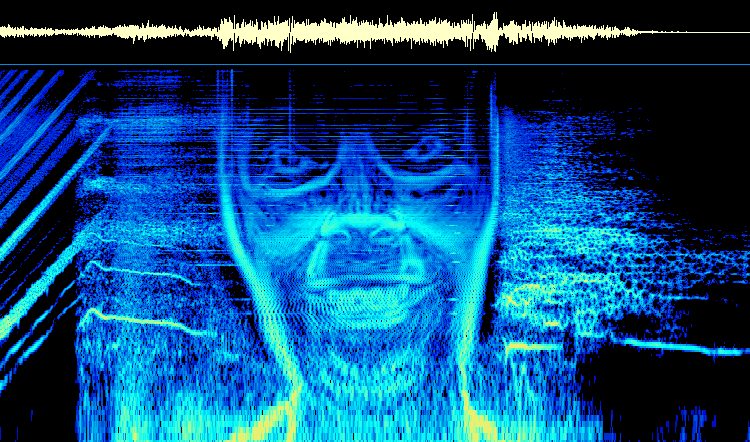
\includegraphics[width = 14cm]{img/aphexFFT.png}
		\caption{Image in the spectrogram in a track by ``Aphex Twin''.}
		\label{fig:Aphex}
	\end{center}
\end{figure}




\begin{center}
\begin{figure}[H]
\tikzset{concept/.append style={fill={none}}}
\begin{tikzpicture}
  \path[mindmap,concept color=black,text=black]
	node[concept] {Fourier Tansform}
	[clockwise from=0]
	% child[concept color=green!50!black] {
	% node[concept] {schuluebung v. letzem Mal}
	% }
	% child[concept color=green!50!black] {node[concept] {pd parxis}
	% 	child[concept color=green!50!black] {node[concept] {send/receive}}
	% 	child[concept color=green!50!black] {node[concept] {initialisierung}}
	% 	}
	% child[concept color=blue] {
	% node[concept] {hauptteil FFT}
	% [clockwise from=-90]
		child[concept color=orange] { node[concept] {theory} }
		child[concept color=red] { node[concept] {practice}
			child[concept color=red] { node[concept] {spectrum display} }
			child[concept color=red] { node[concept] {fft filter}
				child[concept color=red] { node[concept] {random filter} }
				}
			child[concept color=red] { node[concept] {fft reverb} }
			child[concept color=red] { node[concept] {pitch shift} }
		}


;
\end{tikzpicture}
\caption{Lecture Contents: Fourier Transform}
\end{figure}
\end{center}

\section{Further Information}

\begin{itemize}
	\item \link{https://www.youtube.com/watch?v=-IJuqR6nz\_Q}{complex Numbers}
	\item \link{https://www.youtube.com/watch?v=EIstpPXKWng}{The Imaginary Number}
	\item \link{http://jackschaedler.github.io/circles-sines-signals}{Interactive Visualization of the Fourier Transform}

\end{itemize}

% vorbereitung:\\
% Eulers identity, complex numbers.



% Initialisierung
% Fourier transformation.
% Spectral filter
% Spectral Reverb, delay.
% Windowing
% Convolution,
% evtl. cross correlation
% freq. crossover
% spectral synyth,
% spectraum display.


% evtl auch:
% \begin{itemize}
% 	\item send / receive, send / receive bei gui objekten.
% 	\item initialisierung
% 	\item
% \end{itemize}


% Diskretes Signal -> Periodisches Spectrum \\
% Periodisches Signal -> Diskretes Spectrum



% fftuebung
% beiwerk:
	% initialisierung
	% send/receive
% schuluebung von letzem mal
% hauttteil fft
	% theorie	> geschichte
	% praxis
		% spectrum display
		% fft filter
			% nomral
			% random
		% fftdelay
		% fft reverb
		% pitch shift


\section{Fourier Transformation}
\subsection{Concept}
The Fourier transform is a way to switch domains. What does that mean? We can think of it as transforming a piece of information into another representation without loss of information. To give an analogy: \\
If I tell you, we meet at \textit{Matthias Corvinus-Straße 15, 3100 St. Pölten} is the same as telling you we meet at GPS coordinates 48.2138731, 15.6320195. It is the same information in another format, another \textit{domain}.\\
These two formats have different advantages and disadvantages. For example, would you know if the location in GSP format is in Austria? Probably not. On the other hand, the GSP coordinates can theoretically have a lot more precision. Do we meet at the back entrance? Where exactly? What if they decide to change the street name? \\
The point is, depending on what we want, different representations offer different possibilities and insights.
\begin{figure}[H]
	\centering
	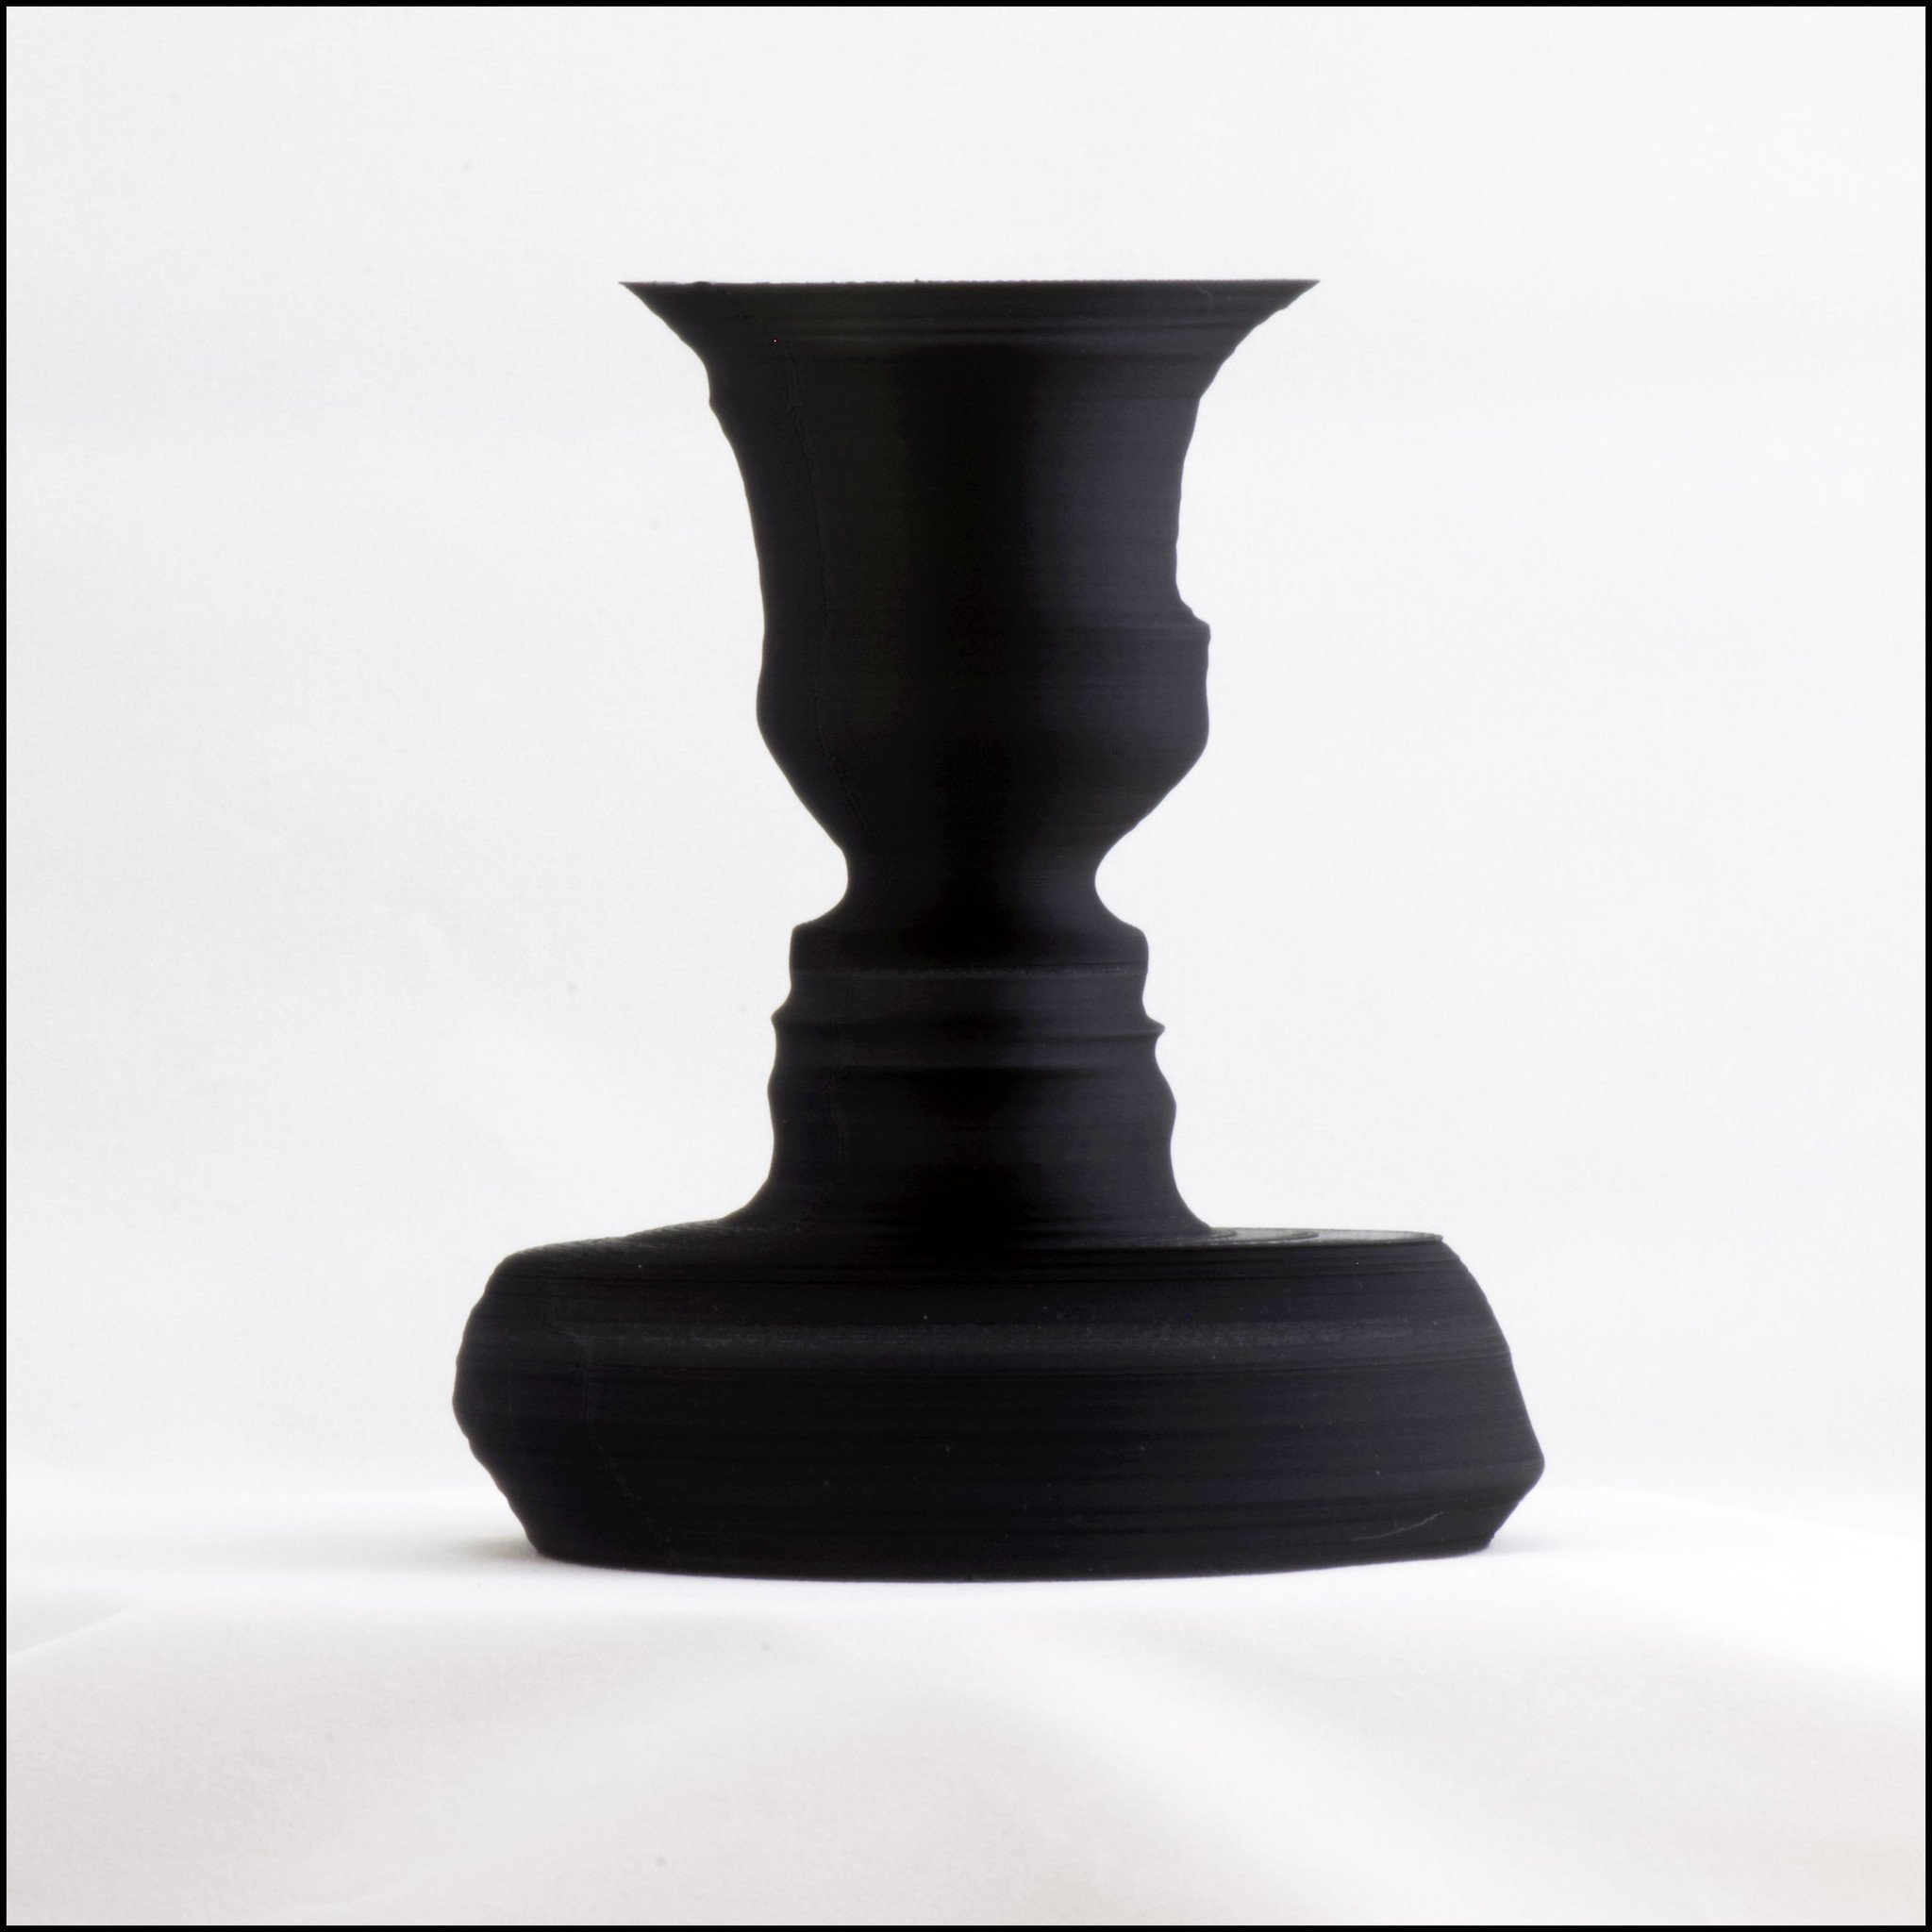
\includegraphics[width=\textwidth]{img/vase.jpg}
	\caption[illusion]
	{Depending on how you look at something, different possibilities and insights arise.}
	\label{fig:vase}
\end{figure}

In the case of the Fourier transform we want to switch to a spectral domain. We want to do this since it would enable us to immediately see if there is a lot of energy at a certain frequency. Oddly, with light in the physical world, this seems very simple, just take a prism:

\begin{figure}[H]
	\centering
	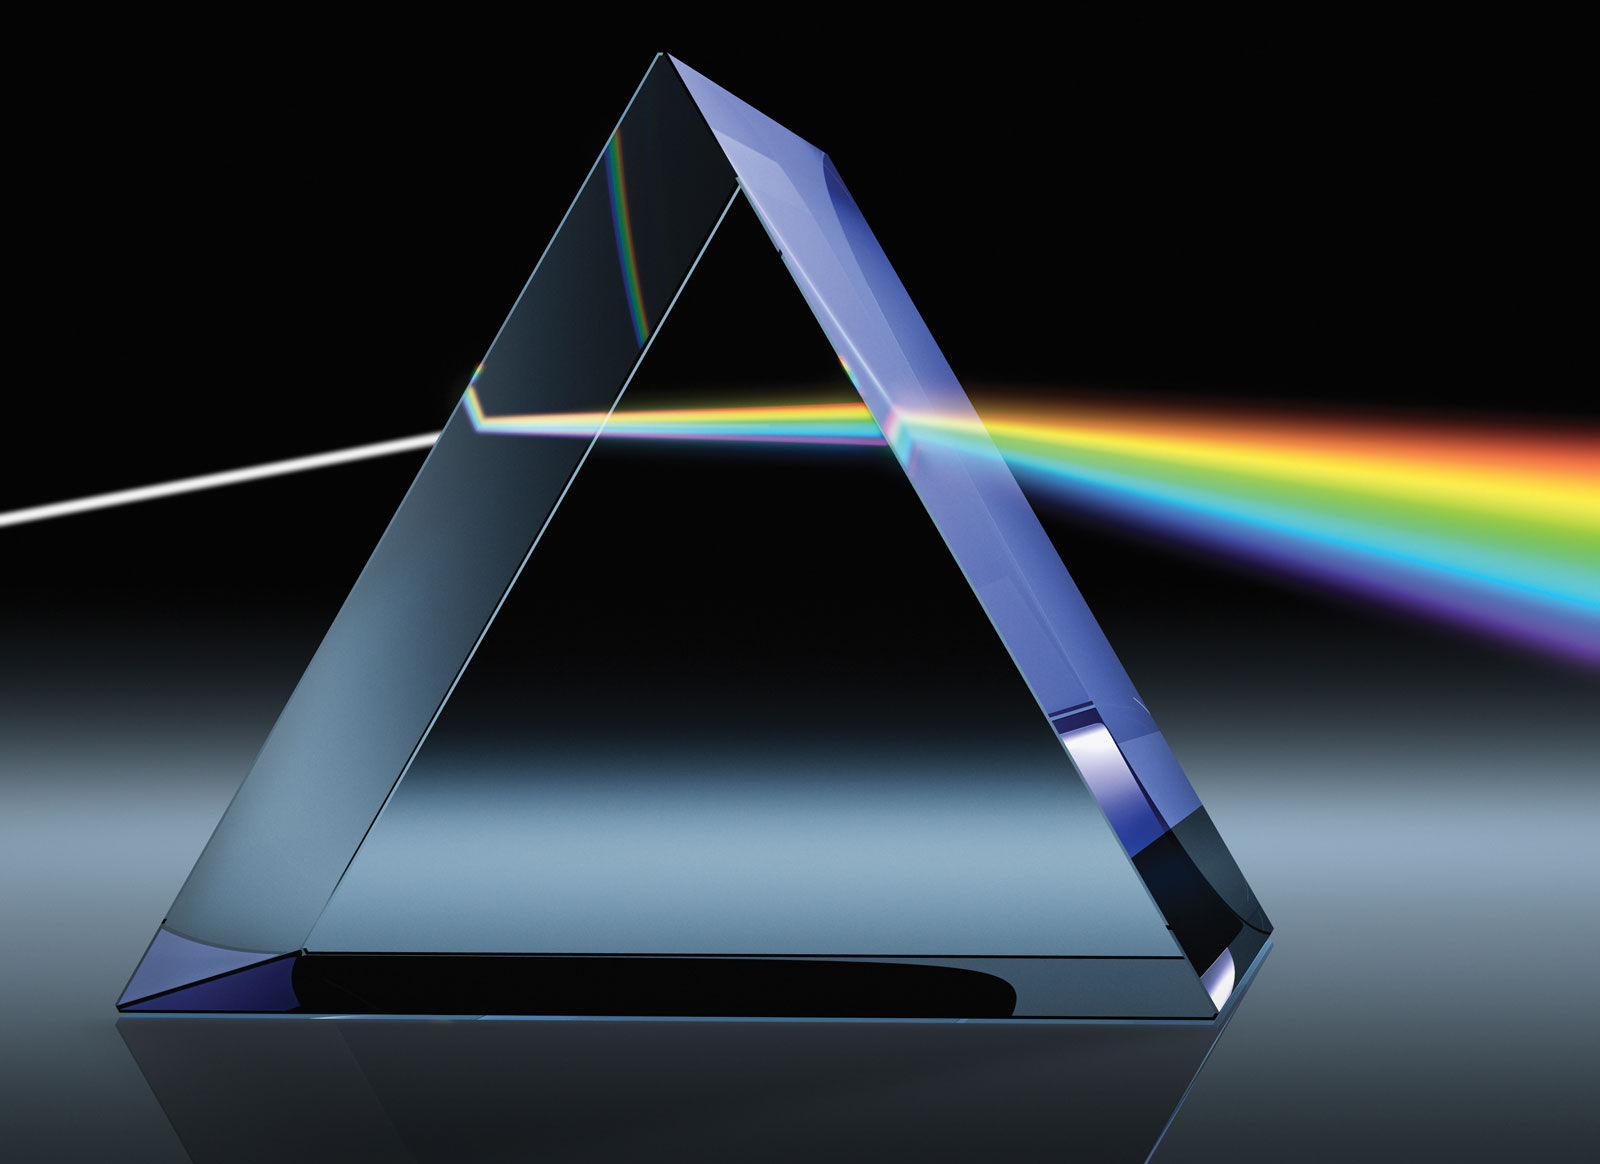
\includegraphics[width=\textwidth]{img/Prism.jpg}
	\caption[prism]
	{A prism splits up light into its different spectral components, essentially performing a Fourier transform.}
	\label{fig:prism}
\end{figure}

\subsection{Math}
So how do we do this domain switching? There are different approaches to explaining what's happening in the Fourier Transform, but I think this is the most intuitive one: Remember, we just want to know how much of a certain frequency is contained in a certain signal $x(t)$.\\
If I give you 100 Euros and ask you to tell me how many 5 Euro bills are "in there", what would you do? Divide, of course. So can we just take a time domain signal and divide it by a sine at some frequency to see how much of it is contained in that signal? Yes!\\
The Fourier transform is defined as

\begin{equation}
	X(f)= \mathcal{F} \{x(t)\} = \int_{-\infty}^\infty \! x(t) e^{-i2\pi ft} \, \mathrm{d}t
	\label{ft}
\end{equation}

Most of the time we are dealing with discrete (digital) signals, but since the  \textit{Discrete Fourier Transform} (DFT) is a bit less intuitive, let's stick to the continuous('analog') one.


What does Equation \ref{ft} mean? We have an input time domain signal $x(t)$. We get out a frequency domain signal $X(f)$. In order to see why this is working, we need to remember Euler's identity:

\begin{equation}
	e ^{ix} = cos(x)+i \cdot sin(x)
\end{equation}

So, the Fourier transform actually is an integral (a continuous summation) over the input signal times cosine and sine terms:


\begin{equation}
	X(f)= \mathcal{F} \{x(t)\} = \int_{-\infty}^\infty \! x(t) \cdot (cos(2\pi ft)+i \cdot sin(2\pi ft) )^{-1}  \, \mathrm{d}t
	\label{ft2}
\end{equation}

And, knowing that a negative exponent means the same as using the reciprocal, so dividing, we can rearrange to:


\begin{equation}
	X(f)= \mathcal{F} \{x(t)\} = \int_{-\infty}^\infty \! \frac{x(t)} { cos(2\pi ft)+i \cdot sin(2\pi ft) }  \, \mathrm{d}t
	\label{ft2}
\end{equation}

Now you can probably see that we just take the input signal, and for each frequency $f$, we just "sum" over the whole input signal to see how much sine and cosine of that frequency is contained. Ok, it's complex sinusoids, we didn't touch on complex numbers etc, but this should give you a feeling why this can work.

% \begin{equation}
% 	x_f(m) = \sum_{n=0}^{N-1} x(n)\cdot (cos(2 \pi \frac{n m}{N})+i \cdot sin(2 \pi \frac{n m}{N}))^{-1}
% \end{equation}


For the sake of completeness, here are some variants of the whole scheme:\\
% Geschichte:
% Bernoulli, Euler, Gauß, Fourier
The discrete Fourier Transform (DFT) is defined as:
\begin{equation}
	x_f(m) = \sum_{n=0}^{N-1} x(n)\cdot e^{-i 2 \pi \frac{n m}{N} }
\end{equation}


Inverse Fourier Transformation:\\
\begin{equation}
	x(t)= \mathcal{F}^{-1} \{X(f)\} = \int_{-\infty}^\infty \! X(f) e^{j2\pi ft} \, \mathrm{d}f
\end{equation}

\subsection{Implementation}

\newpage
As python code this could look like this:
\lstinputlisting[language=Python,caption={DFT in python},captionpos=b]{code/fourierTransform.py}
Beware that the python code above implements the formula directly. It is \textit{very} slow. Typically, a different algorithm is used, such as an implementation of the Fast Fourier Transform (FFT). In python, there are several ways to compute an FFT in an efficient way such as \texttt{numpy.fft.fft()}. The FFT is a classic \textit{divide and conquer} solution to performance boosting an algorithm.


\subsection{Application in pd}
\begin{figure}[h]
	\begin{center}
		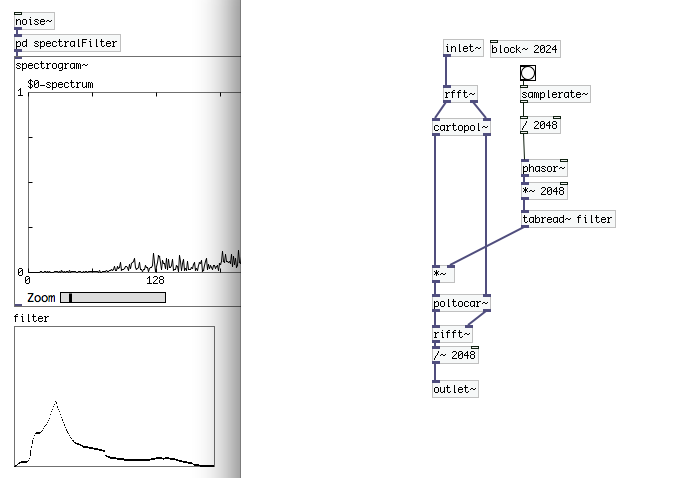
\includegraphics[width = 14cm]{img/spectralFilter.png}
		\caption{spectralFilter.pd}
		\label{fig:spectralFilter}
	\end{center}
\end{figure}

\begin{figure}[h]
	\begin{center}
		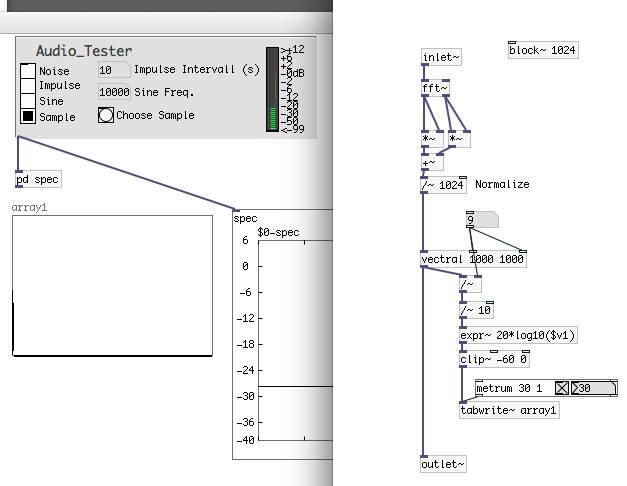
\includegraphics[width = 14cm]{img/showspectrum.png}
		\caption{showspectrum}
		\label{fig:showspectrum}
	\end{center}
\end{figure}
